\documentclass{article}
\usepackage[utf8]{inputenc}

\usepackage{tikz}
\usepackage{tikz-3dplot}
\usetikzlibrary{math}
\usepackage{tkz-euclide}
\usepackage{amsmath, amsthm, amssymb}

\usepackage{polynom}
\polyset{style=C, div=:, vars=x}
\title{Geometría del espacio}
\author{javalejan12 }
\date{July 2022}

\begin{document}

\maketitle

\section{Figuras 3D}
\subsection{Pirámide}

\begin{figure}[h]
    \centering

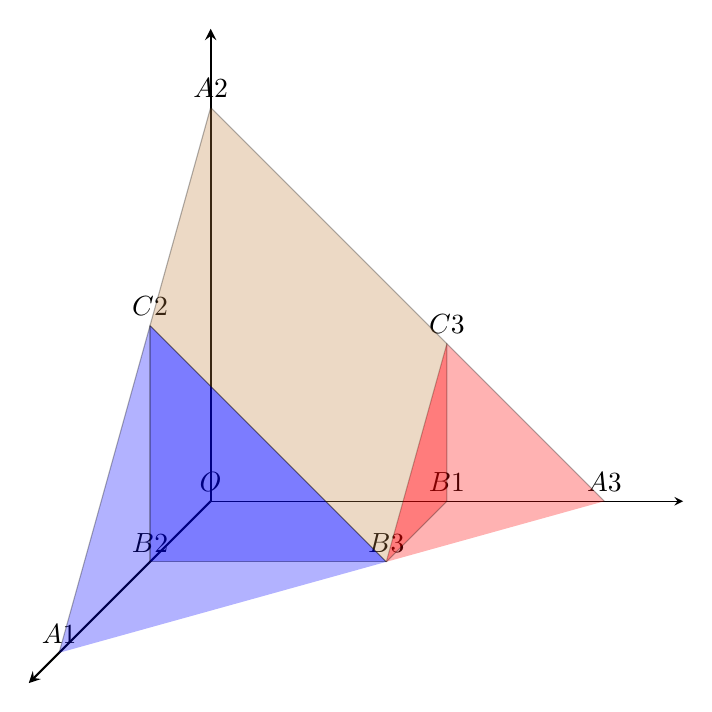
\begin{tikzpicture}
\draw[thick,-stealth] (0,0,0)--(0,0,6); 
\draw[thick,-stealth] (0,0,0)--(0,6,0);
\draw[-stealth] (0,0,0)--(6,0,0);
\coordinate[label=$O$] (O) at (0,0,0);
\coordinate[label=$A1$] (A1) at (0,0,5);
\coordinate[label=$A2$] (A2) at (0,5,0);
\coordinate[label=$A3$] (A3) at (5,0,0);
\coordinate[label=$B1$] (B1) at (3,0,0);
\coordinate[label=$B2$] (B2) at (0,0,2);
\coordinate[label=$B3$] (B3) at (3,0,2);
\coordinate[label=$C2$] (C2) at (0,3,2);
\coordinate[label=$C3$] (C3) at (3,2,0);

\draw[fill=blue,opacity=0.3] (A1)--(C2)--(B3);
draw[fill=black,opacity=0.3] (O)--(B2)--(B3)--(B1)
\draw[fill=red,opacity=0.3] (A3)--(C3)--(B3);
\draw[fill=red,opacity=0.3] (B3)--(B1)--(C3);
\draw[fill=blue,opacity=0.3] (C2)--(B2)--(B3);
\draw[fill=brown,opacity=0.3] (B3)--(C2)--(A2)--(C3);
\end{tikzpicture}
\end{figure}

\subsubsection{Tronco de pirámide}
Sea el tronco de pirámide de altura $h$.\\ 

\begin{figure}[h]
    \centering
    \centering
	\tdplotsetmaincoords{60}{110}


\begin{tikzpicture}[tdplot_main_coords,scale=1]
\coordinate[label=$A1$] (A1) at (0,0,5);
\coordinate[label=$A2$] (A2) at (2,3,5);
\coordinate[label=$A3$] (A3) at (5,3,5);
\coordinate[label=$A4$] (A4) at (7,0,5);
\draw[fill=blue,opacity=0.3] (A1)--(A2)--(A3)--(A4);
\coordinate[label=$B1$] (B1) at  (-2.333333,-1,0);
\coordinate[label=$B2$] (B2) at (1,4,0);
\coordinate[label=$B3$] (B3) at (6,4,0);
\coordinate[label=$B4$] (B4) at (9.333333,-1,0);
\draw[color=black,fill=red,opacity=0.3] (B1)--(B2)--(B3)--(B4);
\draw[dashed,color=gray] (A1)--(B1);
\draw (A2)--(B2);
\draw (A3)--(B3);
\draw (A4)--(B4);
\draw (A1)--(A2)--(A3)--(A4)--cycle;
\draw (B2)--(B3)--(B4);
\draw[dashed,color=gray] (B4)--(B1)--(B2);
\coordinate (E) at (intersection of A1--A3 and A2--A4);
\coordinate (F) at (intersection of B1--B3 and B2--B4);
\draw[dashed,color=blue] (E)--(F);
\tkzLabelSegment[left](E,F){$h$}
\end{tikzpicture}\end{figure}
Su volumen está dado por:
\begin{equation*}
    V = \dfrac{h}{3}  (A_{A1234} + A_{B1234}+\sqrt{A_{A1234} A_{B1234} })
\end{equation*}

$$\polylongdiv{x^4+3x^3-2x^2+x-1}{x^2+x-1}$$
\end{document}
